\documentclass[11pt]{article}

\usepackage[margin=1in]{geometry}
\usepackage{graphicx}
\usepackage{booktabs}
\usepackage{caption}
\usepackage{subcaption}
\usepackage{authblk}
\usepackage{lineno}
\usepackage[numbers,super,sort&compress]{natbib}
\usepackage{hyperref}
\usepackage{microtype}

\graphicspath{{figures/}}

\hypersetup{
  colorlinks=true,
  linkcolor=black,
  citecolor=black,
  urlcolor=black
}

\linenumbers

% Overleaf upload checklist:
% 1. Upload this file as main.tex, or set this file as the main document.
% 2. Upload manuscript/figures/ as an Overleaf folder named figures/.
% 3. Required figure files:
%    figures/figure_1_framework.pdf
%    figures/figure_2_primary_background_audit.pdf
%    figures/figure_4_cross_resistance_network.pdf
%    figures/figure_5_public_wgs_proteomic_support.pdf

\title{\bfseries A Background-Matched Audit Reveals Co-resistance Background Sensitivity in MALDI-TOF AMR Prediction}

\author[1]{Byung Kim}
\author[2]{Yucheng Wang}
\author[3]{Nicolas Samuel Khoury-Levy}
\affil[1]{United States Air Force Academy, Colorado Springs, CO, USA}
\affil[2]{University of Wisconsin--Madison, Madison, WI, USA}
\affil[3]{Cornell University, Ithaca, NY, USA}
\date{}

\begin{document}
\maketitle

\begin{abstract}
Machine learning models trained on matrix-assisted laser desorption/ionization time-of-flight (MALDI-TOF) spectra can predict antimicrobial resistance (AMR), but raw external AUC does not reveal whether prediction reflects focal resistance biology or the spectral background of resistant bacterial populations. We developed a model-agnostic background-matched audit that evaluates isolate-level predictions within matched co-resistance strata. Applied to \textit{Escherichia coli} DRIAMS models trained at DRIAMS-A and tested temporally and across external hospitals, ciprofloxacin raw AUCs of 0.823, 0.750, and 0.671 at A-2018, DRIAMS-C, and DRIAMS-D attenuated to background-centered AUCs of 0.703, 0.646, and 0.596. Amoxicillin-clavulanic acid raw AUCs of 0.650, 0.535, and 0.557 at the same sites weakened or collapsed to centered AUCs of 0.541, 0.497, and 0.486. In a second organism-drug setting, \textit{Staphylococcus aureus}/oxacillin retained background-matched signal at the evaluable DRIAMS sites, with raw AUCs of 0.838, 0.775, and 0.725 and centered AUCs of 0.763, 0.864, and 0.699 at A-2018, DRIAMS-B, and DRIAMS-C. Exact co-resistance-only baselines showed that non-focal AST labels alone could strongly predict several \textit{E.~coli} targets, including DRIAMS-C ciprofloxacin (AUC 0.918) and amoxicillin-clavulanic acid (AUC 0.687), whereas \textit{S.~aureus}/oxacillin retained MALDI signal competitive with or above the AST-only baseline at A-2018 and DRIAMS-C. Background-matched evaluation provides a practical guardrail for MALDI-TOF AMR studies by distinguishing aggregate transfer from focal-drug signal that survives within resistant-population background.
\end{abstract}

\section*{Significance}

MALDI-TOF instruments are already present in clinical microbiology laboratories, making AMR prediction from routine spectra attractive. The central risk is that a model may appear to predict resistance while partly detecting the resistant clone, co-resistance block, or hospital ecology in which resistance is concentrated. That distinction matters for deployment: a shortcut that works in one hospital can fail when local resistant populations change. This study converts that concern into an operational audit requiring only ordinary model predictions and AST labels. The audit does not prove mechanism, but it shows whether a claimed drug prediction survives within matched co-resistance backgrounds and whether ordinary AST co-resistance labels alone can explain much of the apparent signal. This makes MALDI-TOF AMR evaluation more interpretable, more reproducible, and safer to compare across organisms and sites.

\section*{Introduction}

Rapid antimicrobial susceptibility information is central to effective treatment and stewardship\cite{murray2022amr}. MALDI-TOF mass spectrometry is already used at scale for bacterial identification\cite{seng2009maldi,patel2015maldi}, and several studies have shown that the same spectra can support machine-learning prediction of AMR\cite{weis2022driams,msdeepamr2024,multilabel2024,saureus2024}. The DRIAMS resource was especially important because it paired clinical MALDI-TOF spectra with susceptibility labels across multiple hospitals and demonstrated that AMR prediction can transfer beyond a single laboratory under some organism-drug settings\cite{weis2022driams,driamsdryad}. That result created a realistic translational question: not whether MALDI-TOF spectra contain predictive information, but what biological and population signals that information represents.

A resistance label is not an isolated molecular state. In clinical bacterial populations, resistance is often concentrated in disseminated lineages, plasmid backgrounds, and co-resistance blocks\cite{canton2011coresistance,pal2015coselection}. These structures vary by hospital and sampling period. A model trained to separate resistant from susceptible isolates can therefore succeed by learning any spectral correlate of resistance, including lineage-associated protein peaks that are not the focal resistance mechanism. This risk is not hypothetical. Yu \textit{et al.} recently showed that biased sampling and bacterial population structure can confound WGS-based machine-learning AMR prediction across multiple pathogens\cite{yu2025population}. We ask whether the analogous problem arises in MALDI-TOF spectra, where routine spectra can encode phylogenetic and strain background because conserved proteins vary across lineages.

For clinical translation, the usual question, ``What is the external AUC?'', is incomplete. A high external AUC can arise when the training and test sites share a resistant subpopulation, even if the model is using background structure rather than focal-drug biology. Conversely, an external AUC can decline when the resistant population changes, even if the model learned a real signal that is not represented in the new site. AUC alone does not distinguish these cases. This gap is adjacent to, but not covered by, general clinical prediction-model reporting and bias tools such as TRIPOD+AI and PROBAST\cite{collins2024tripodai,wolff2019probast}. Those frameworks specify transparent reporting and risk-of-bias assessment for prediction models; they do not provide a MALDI-AMR-specific test for whether apparent drug prediction survives resistant-population background.

The closest MALDI-TOF precedent is the hierarchical stratification approach of Weis \textit{et al.}, which partitions data by spectral similarity to evaluate AMR models under more stringent background-aware splits\cite{weis2022stratification}. Our audit is complementary rather than redundant. Hierarchical stratification is spectrum-level and split-level: it requires raw spectra or spectral distances and is naturally tied to the data representation used for evaluation. The background-matched audit is prediction-table-level and post hoc: it requires only isolate identifiers, site, drug, AST label, model probability, and the AST panel used to construct co-resistance backgrounds. It can therefore be run by an independent auditor on predictions from a CNN, gradient-boosted model, logistic regression workflow, or future deployed system without raw spectra or model internals.

We introduce a background-matched MALDI-AMR audit. For each focal drug, the method groups isolates by the AST labels of the other drugs in the panel, then asks whether model predictions still separate resistant from susceptible isolates within those matched co-resistance backgrounds. The design follows the logic of matched observational analyses: evaluate treated and untreated units, here resistant and susceptible isolates, inside comparable background strata rather than relying only on aggregate comparisons\cite{rosenbaum1983propensity}. It produces raw AUC, matched AUC, background-centered AUC, pairwise within-background accuracy, matched retention, and adequacy flags for each drug-site row.

We apply this framework first to an expanded \textit{E.~coli} DRIAMS panel and focus the main evidence on a contrast between ciprofloxacin and amoxicillin-clavulanic acid. Ciprofloxacin resistance in \textit{E.~coli} is strongly linked to globally disseminated lineages, especially ST131, whereas amoxicillin-clavulanic acid resistance is more ecologically heterogeneous\cite{nicolas2014st131}. We then apply the same audit to \textit{S.~aureus}/oxacillin as a second organism-drug setting, test whether the same audit behavior appears across model families, compare MALDI model outputs with co-resistance-only baselines, examine the co-resistance network that models can exploit, and use independent public WGS-linked MALDI data to ask whether lineage-associated spectral shortcuts are biologically plausible.

\section*{Results}

\subsection*{Raw external performance did not identify the source of signal}

We first evaluated raw external performance for a DRIAMS-A-trained \textit{E.~coli} MALDI-AMR model across a temporal DRIAMS-A 2018 holdout and external DRIAMS-B, DRIAMS-C, and DRIAMS-D test sites. The six-drug panel included ciprofloxacin, norfloxacin, amoxicillin-clavulanic acid, ceftriaxone, ceftazidime, and cefepime. Raw AUCs were heterogeneous across drugs and sites. At A-2018, AUC ranged from 0.650 for amoxicillin-clavulanic acid to 0.867 for cefepime; ciprofloxacin reached 0.823. At DRIAMS-C and DRIAMS-D, ciprofloxacin raw AUCs were 0.750 and 0.671, while amoxicillin-clavulanic acid raw AUCs were 0.535 and 0.557.

These values describe aggregate transfer, but they do not identify what the model used to transfer. In a panel where resistance phenotypes are correlated, a model can assign higher scores to isolates from a resistant background even when it does not rank resistant isolates above susceptible isolates within the same background. This is the central distinction tested by the background-matched audit.

\subsection*{The audit measured prediction inside matched co-resistance backgrounds}

For each focal drug, we constructed a co-resistance signature from all non-focal drug AST labels in the same organism panel. Isolates with the same signature formed a background stratum. A valid stratum required at least three resistant and three susceptible isolates for the focal drug. Within each site-drug row, we computed four performance summaries. Raw AUC used all available isolates. Matched AUC restricted evaluation to valid strata. Background-centered AUC subtracted the mean model score within each valid stratum before pooling residual scores and recomputing AUC. Pairwise within-background accuracy counted only resistant-susceptible pairs drawn from the same valid stratum, with ties counted as 0.5.

The distinction between the last two statistics is important. Background-centered AUC removes stratum-level score shifts but remains a pooled residual AUC. Pairwise within-background accuracy is the direct within-stratum statistic. We therefore report both, together with matched retention and adequacy flags. Low retention is not interpreted as biological failure; it is reported as an audit limitation because the dataset does not contain enough matched resistant-susceptible comparisons to support a strong conclusion (Fig.~\ref{fig:framework}).

\begin{figure}[ht]
\centering
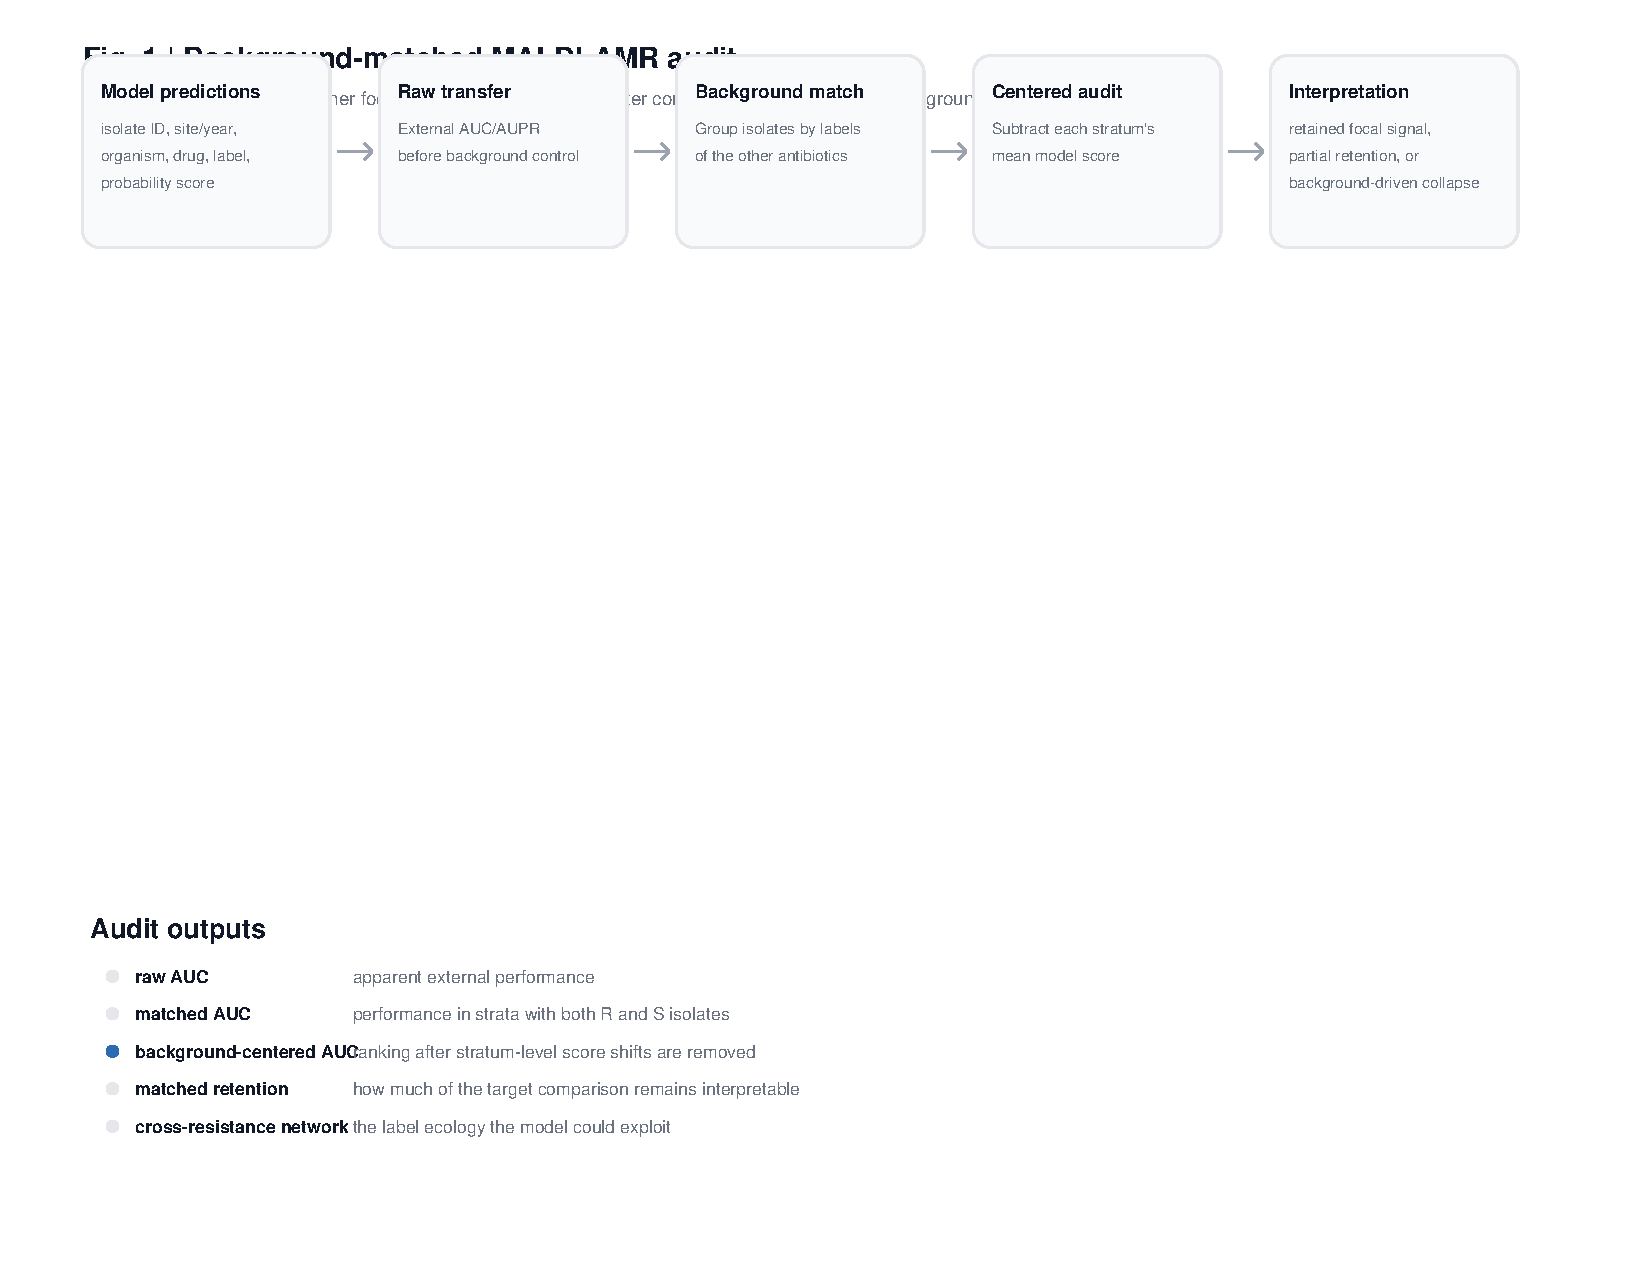
\includegraphics[width=\linewidth]{figure_1_framework.pdf}
\caption{\textbf{Background-matched audit workflow.} The audit accepts isolate-level prediction rows from any MALDI-TOF AMR model. For each focal drug, non-focal AST labels define a co-resistance background signature. Valid strata contain at least three resistant and three susceptible isolates for the focal drug. The audit reports raw AUC, matched AUC, background-centered AUC, pairwise within-background accuracy, matched retention, and adequacy labels.}
\label{fig:framework}
\end{figure}

\subsection*{Ciprofloxacin retained partial signal after matching, whereas amoxicillin-clavulanic acid collapsed externally}

The primary comparison was \textit{E.~coli}/ciprofloxacin versus \textit{E.~coli}/amoxicillin-clavulanic acid. The two drugs were evaluated with the same training site, model pipeline, organism, and external sites, but they differed in resistant-population ecology.

Ciprofloxacin retained residual discrimination after background matching at the main interpretable sites, but the strength of retention was site dependent. Background-centered AUC was 0.703 at A-2018 and 0.646 at DRIAMS-C, consistent with retained within-background ranking. At DRIAMS-D, centered AUC was lower at 0.596 (95\% CI 0.565--0.624), indicating weak but nonzero residual discrimination rather than strong transfer. The direct within-background statistic agreed with this pattern: pairwise within-background accuracy was 0.754, 0.675, and 0.616 at A-2018, DRIAMS-C, and DRIAMS-D. DRIAMS-B had a high centered estimate, but it was based on only 25 matched isolates and one valid stratum with a wide confidence interval; we therefore interpret DRIAMS-B as statistically uninformative for ciprofloxacin rather than as evidence of strong retention.

Amoxicillin-clavulanic acid behaved differently. At A-2018, the model showed only weak residual signal after centering, with centered AUC 0.541. At DRIAMS-C and DRIAMS-D, centered AUC fell to 0.497 and 0.486 despite high matched retention, and pairwise within-background accuracy fell to chance or below chance. DRIAMS-B again provided only uncertain support. Thus, the contrast was not simply that one drug had higher raw AUC than another. The key result is that ciprofloxacin retained partial ranking information inside matched backgrounds, whereas amoxicillin-clavulanic acid did not retain meaningful external within-background signal (Fig.~\ref{fig:primary}; Table~\ref{tab:primary-audit}).

Because ciprofloxacin and norfloxacin were nearly collinear in the AST network, we explicitly audited the composition of the valid ciprofloxacin background strata. This did not show that valid ciprofloxacin strata were dominated by norfloxacin-susceptible backgrounds. Instead, norfloxacin was unknown in all valid A-2018, DRIAMS-C, and DRIAMS-D ciprofloxacin strata at the main threshold (9/9, 4/4, and 10/10 valid strata, respectively), while the single DRIAMS-B valid stratum was norfloxacin-resistant. Thus, the interpretable ciprofloxacin rows are not a within-fluoroquinolone-pair test. They are a cross-class background test: within beta-lactam and cephalosporin co-resistance backgrounds, the model still retained partial ciprofloxacin discrimination. That makes the retained ciprofloxacin signal more conservative than a comparison controlled only by a near-redundant fluoroquinolone label, while norfloxacin missingness still prevents a fully controlled fluoroquinolone-pair analysis.

We also repeated the audit with stricter valid-stratum thresholds requiring at least five or ten resistant and susceptible isolates per background. The primary contrast was stable. At the threshold of five per class, centered AUCs were 0.705, 0.656, and 0.597 for ciprofloxacin at A-2018, DRIAMS-C, and DRIAMS-D, while amoxicillin-clavulanic acid remained weak or chance-level at 0.539, 0.511, and 0.490. At the threshold of ten per class, DRIAMS-B ciprofloxacin had no valid strata, as expected; A-2018, DRIAMS-C, and DRIAMS-D ciprofloxacin remained above chance (0.743, 0.656, and 0.613), whereas amoxicillin-clavulanic acid remained weak (0.546, 0.475, and 0.492). These analyses support the contrast while showing that the DRIAMS-D ciprofloxacin effect is modest.

\begin{figure}[ht]
\centering
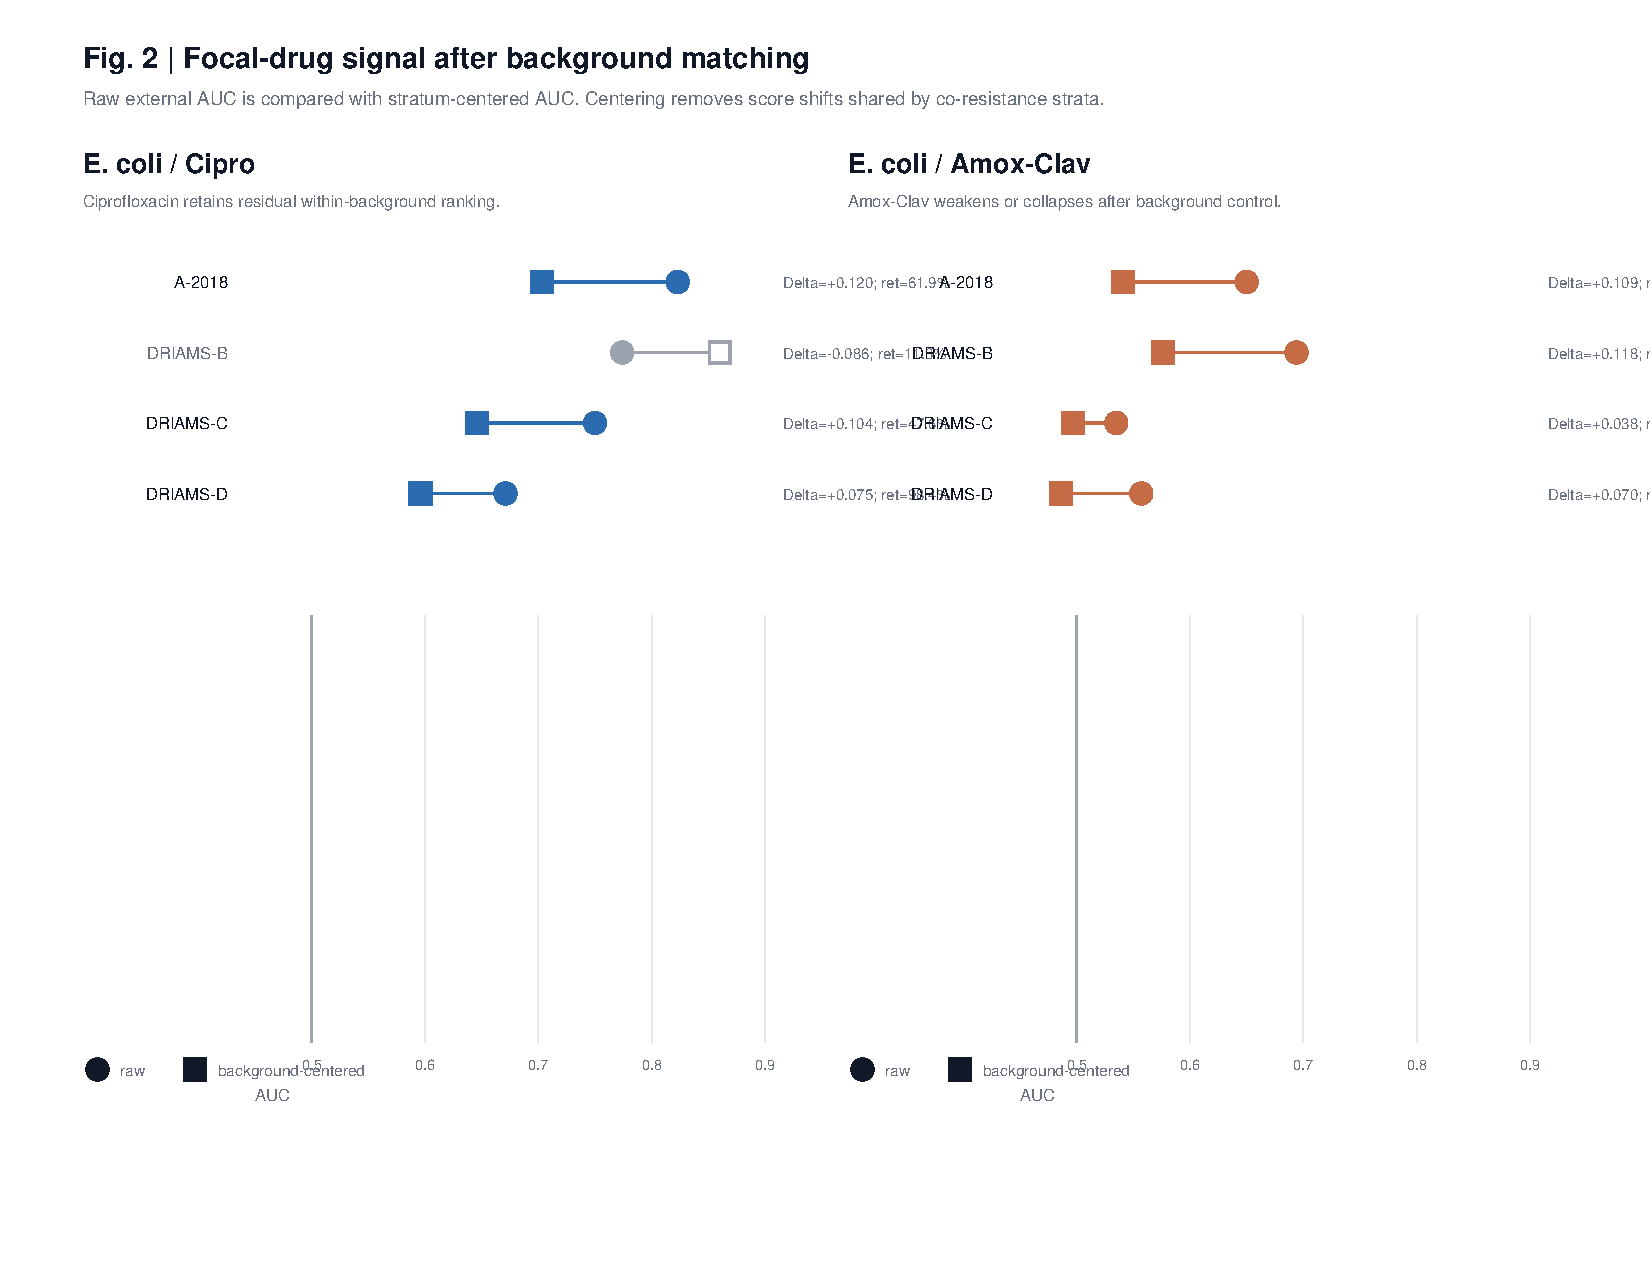
\includegraphics[width=\linewidth]{figure_2_primary_background_audit.pdf}
\caption{\textbf{Primary background-matched audit.} Raw and background-centered AUCs for \textit{E.~coli}/ciprofloxacin and \textit{E.~coli}/amoxicillin-clavulanic acid across temporal and external DRIAMS sites. Ciprofloxacin retains residual within-background discrimination at the main interpretable sites, whereas amoxicillin-clavulanic acid weakens or collapses toward chance externally. Rows with low matched support are flagged rather than treated as primary evidence.}
\label{fig:primary}
\end{figure}

\begin{table}[ht]
\centering
\small
\caption{\textbf{Primary background-matched audit rows.} Centered AUC is computed after subtracting the mean model score within each co-resistance background stratum. Caution rows are reported but not used as primary evidence.}
\label{tab:primary-audit}
\resizebox{\linewidth}{!}{%
\begin{tabular}{llccccccl}
\toprule
Pair & Site & Raw AUC & Centered AUC & Retention (\%) & $n$ matched & Valid strata & $P_{\mathrm{perm}}$ & Interpretation \\
\midrule
\textit{E.~coli}/Cipro & A-2018 & 0.823 (0.799--0.849) & 0.703 (0.664--0.747) & 61.9 & 836 & 9 & 0.002 & Retained signal \\
\textit{E.~coli}/Cipro & DRIAMS-B & 0.774 (0.692--0.841) & 0.860 (0.636--1.000) & 11.8 & 25 & 1 & 0.010 & Caution; low support \\
\textit{E.~coli}/Cipro & DRIAMS-C & 0.750 (0.702--0.795) & 0.646 (0.576--0.719) & 47.6 & 422 & 4 & 0.002 & Retained signal \\
\textit{E.~coli}/Cipro & DRIAMS-D & 0.671 (0.640--0.700) & 0.596 (0.565--0.624) & 98.4 & 1908 & 10 & 0.002 & Weak retained signal \\
\textit{E.~coli}/Amox--Clav & A-2018 & 0.650 (0.619--0.685) & 0.541 (0.504--0.576) & 92.2 & 1261 & 14 & 0.038 & Weak residual signal \\
\textit{E.~coli}/Amox--Clav & DRIAMS-B & 0.694 (0.611--0.765) & 0.576 (0.410--0.715) & 62.1 & 123 & 1 & 0.204 & Weak or uncertain \\
\textit{E.~coli}/Amox--Clav & DRIAMS-C & 0.535 (0.494--0.577) & 0.497 (0.449--0.547) & 89.2 & 805 & 10 & 0.675 & Near chance \\
\textit{E.~coli}/Amox--Clav & DRIAMS-D & 0.557 (0.521--0.590) & 0.486 (0.450--0.521) & 97.4 & 1943 & 11 & 0.854 & Near chance \\
\bottomrule
\end{tabular}%
}
\end{table}

\subsection*{\textit{S.~aureus}/oxacillin retained signal in a second organism-drug setting}

We next applied the same audit to a seven-drug \textit{S.~aureus} panel with oxacillin as the primary target. Oxacillin was evaluable at A-2018, DRIAMS-B, and DRIAMS-C; the DRIAMS-D export contained \textit{S.~aureus} predictions for other drugs but no usable oxacillin focal rows, so DRIAMS-D was not used for the oxacillin claim.

Unlike the \textit{E.~coli}/amoxicillin-clavulanic acid rows that collapsed after matching, \textit{S.~aureus}/oxacillin retained substantial background-matched signal across the evaluable sites. Raw AUCs were 0.838, 0.775, and 0.725 at A-2018, DRIAMS-B, and DRIAMS-C. Background-centered AUCs were 0.763, 0.864, and 0.699, with pairwise within-background accuracies of 0.770, 0.864, and 0.719 (Table~\ref{tab:saureus-oxa}). The A-2018 and DRIAMS-C rows also remained interpretable under a stricter threshold requiring at least ten resistant and ten susceptible isolates per valid stratum, with centered AUCs of 0.766 and 0.723. DRIAMS-B became non-interpretable under that stricter threshold, so its high point estimate should be treated as supportive but sparse single-stratum evidence rather than as a precise site-level estimate. This second organism-drug result shows that the audit does not only identify collapse; it can also identify settings in which MALDI predictions retain signal inside matched co-resistance backgrounds.

\begin{table}[ht]
\centering
\small
\caption{\textbf{\textit{S.~aureus}/oxacillin background-matched audit.} Oxacillin retained background-matched signal at the three evaluable DRIAMS sites. DRIAMS-D was not included because the exported panel contained no usable oxacillin focal rows.}
\label{tab:saureus-oxa}
\resizebox{\linewidth}{!}{%
\begin{tabular}{llcccccl}
\toprule
Pair & Site & Raw AUC & Centered AUC & Pairwise accuracy & Retention (\%) & Valid strata & Interpretation \\
\midrule
\textit{S.~aureus}/Oxacillin & A-2018 & 0.838 (0.799--0.876) & 0.763 (0.714--0.808) & 0.770 & 60.1 & 9 & Retained signal \\
\textit{S.~aureus}/Oxacillin & DRIAMS-B & 0.775 (0.649--0.878) & 0.864 (0.775--0.948) & 0.864 & 52.6 & 1 & Retained; sparse support \\
\textit{S.~aureus}/Oxacillin & DRIAMS-C & 0.725 (0.643--0.800) & 0.699 (0.615--0.782) & 0.719 & 59.6 & 2 & Retained signal \\
\bottomrule
\end{tabular}%
}
\end{table}

\subsection*{Co-resistance structure provided an exploitable background}

The audit results were consistent with the structure of the AST panel. Across the \textit{E.~coli} panel, ciprofloxacin and norfloxacin formed an exceptionally strong fluoroquinolone block, with $\phi = 0.976$ and resistant Jaccard similarity $= 0.963$. Extended-spectrum cephalosporins also formed strong co-resistance blocks: ceftriaxone-ceftazidime $\phi = 0.884$, ceftazidime-cefepime $\phi = 0.828$, and ceftriaxone-cefepime $\phi = 0.804$. These correlations are expected in clinical AMR ecology, where co-resistance and co-selection can concentrate multiple resistance phenotypes in the same strains or mobile-element backgrounds\cite{canton2011coresistance,pal2015coselection}. They also mean that a model trained on focal resistance labels is exposed to a broader label ecology in which resistance to one drug often identifies resistance to another.

This structure is exactly the kind of background that can inflate or destabilize raw AUC. If a model assigns higher scores to isolates from a co-resistant population, it can perform well in aggregate even when focal-drug discrimination within matched backgrounds is weak. The cephalosporin rows illustrate the same caution. Several raw AUCs were high, but many matched analyses had low retention or strong attenuation after centering. We therefore report them in the supplementary audit table with explicit retention flags rather than suppressing them or treating them as clean evidence of focal signal.

\subsection*{Co-resistance-only baselines quantified AST-label shortcut structure}

To make the shortcut question explicit, we trained no spectral model at all: for each focal drug, we predicted resistance from the full non-focal AST background signature using a leave-one-out smoothed prevalence score. This exact co-resistance-only baseline uses only other drug labels, never MALDI spectra and never the isolate's own focal label in its score. It therefore estimates how much focal resistance is predictable from AST ecology alone.

The baseline showed that several \textit{E.~coli} targets contain strong AST-label shortcut structure. At DRIAMS-C, for example, exact co-resistance-only AUC was 0.918 for ciprofloxacin and 0.687 for amoxicillin-clavulanic acid. The corresponding MALDI background-centered AUCs were 0.646 and 0.497. At A-2018, exact-background AUC was also high for ciprofloxacin (0.860) and competitive for amoxicillin-clavulanic acid (0.627). These comparisons do not invalidate the MALDI model; they show why raw MALDI AUC alone is insufficient. In some rows, especially \textit{E.~coli} beta-lactams and cephalosporins, the AST background itself predicts the focal label extremely well.

The \textit{S.~aureus}/oxacillin pattern was different. At A-2018, the exact co-resistance-only baseline reached AUC 0.762, while the MALDI model had raw AUC 0.838 and centered AUC 0.763. At DRIAMS-C, the exact-background baseline was 0.627, while the MALDI model retained centered AUC 0.699. DRIAMS-B remained more ambiguous because exact-background AUC was 0.795 and the matched MALDI estimate was based on one valid stratum. Together, these controls sharpen the interpretation: the audit distinguishes rows where raw performance is largely explainable from non-focal AST ecology from rows where MALDI predictions retain additional or competitive within-background signal.

\subsection*{Background sensitivity was not specific to one model architecture}

To test whether the audit result was a neural-network artifact, we applied the same background-matched procedure to convolutional neural network predictions and multi-task LightGBM predictions. The qualitative pattern was shared. In interpretable amoxicillin-clavulanic acid rows, the mean raw-minus-centered drop was 0.084 for the CNN and 0.116 for LightGBM. In interpretable ciprofloxacin rows, the mean background-centered AUC was 0.648 for the CNN and 0.618 for LightGBM. At DRIAMS-C and DRIAMS-D, amoxicillin-clavulanic acid collapsed after matching in both model families, while ciprofloxacin retained partial signal.

This result does not prove that the two architectures learned identical features. It shows something more important for evaluation: background sensitivity persisted when the model family changed. The sensitivity therefore appears to originate in the relationship among spectra, AST labels, and resistant-population ecology, not in a single representation learned by one architecture. This interpretation is also consistent with recent MALDI-AMR transfer-learning and domain-adaptation studies, which show that cross-site performance depends strongly on target-site composition and labeled target-site adaptation\cite{msdeepamr2024,domainadapt2026}. The full model-family comparison is provided as supplementary support.

\subsection*{Public WGS-linked MALDI data supported lineage as a plausible spectral shortcut}

The DRIAMS isolates used in the primary audit do not have linked WGS labels, so the audit cannot directly prove that a specific lineage drove any DRIAMS prediction. We therefore used independent public WGS-linked Basel uropathogenic \textit{E.~coli} data to test a narrower biological premise: can MALDI peak features detect lineage strongly enough to act as a shortcut for resistance prediction?

In 407 isolates with Bruker MALDI peak features and WGS-derived metadata, ST131 lineage identity was predicted from MALDI peak features with AUC 0.932. In the same cohort, ciprofloxacin resistance was predicted with AUC 0.755 and ceftriaxone resistance with AUC 0.689. ST131 was also strongly associated with these resistance phenotypes. Exact sequence-type centering attenuated ciprofloxacin AUC to 0.564 and ceftriaxone AUC to 0.503. Thus, MALDI spectra contained a strong lineage signal, and resistance prediction weakened when fine-grained lineage background was controlled.

We also compared discriminative MALDI bins with published ST131 biomarker masses\cite{nakamura2019st131}. ST131-discriminative bins were enriched for published ST131 biomarker neighborhoods by 3.11-fold. Ciprofloxacin- and ceftriaxone-discriminative bins were also enriched, at 2.24-fold and 2.64-fold, respectively. These are mass-neighborhood overlaps, not protein identifications. They support the plausibility that resistance-associated MALDI features can overlap lineage-associated features, but they do not establish protein identity or prove the same mechanism inside DRIAMS (Fig.~\ref{fig:background-support}).

\begin{figure}[ht]
\centering
\begin{subfigure}{0.48\linewidth}
\centering
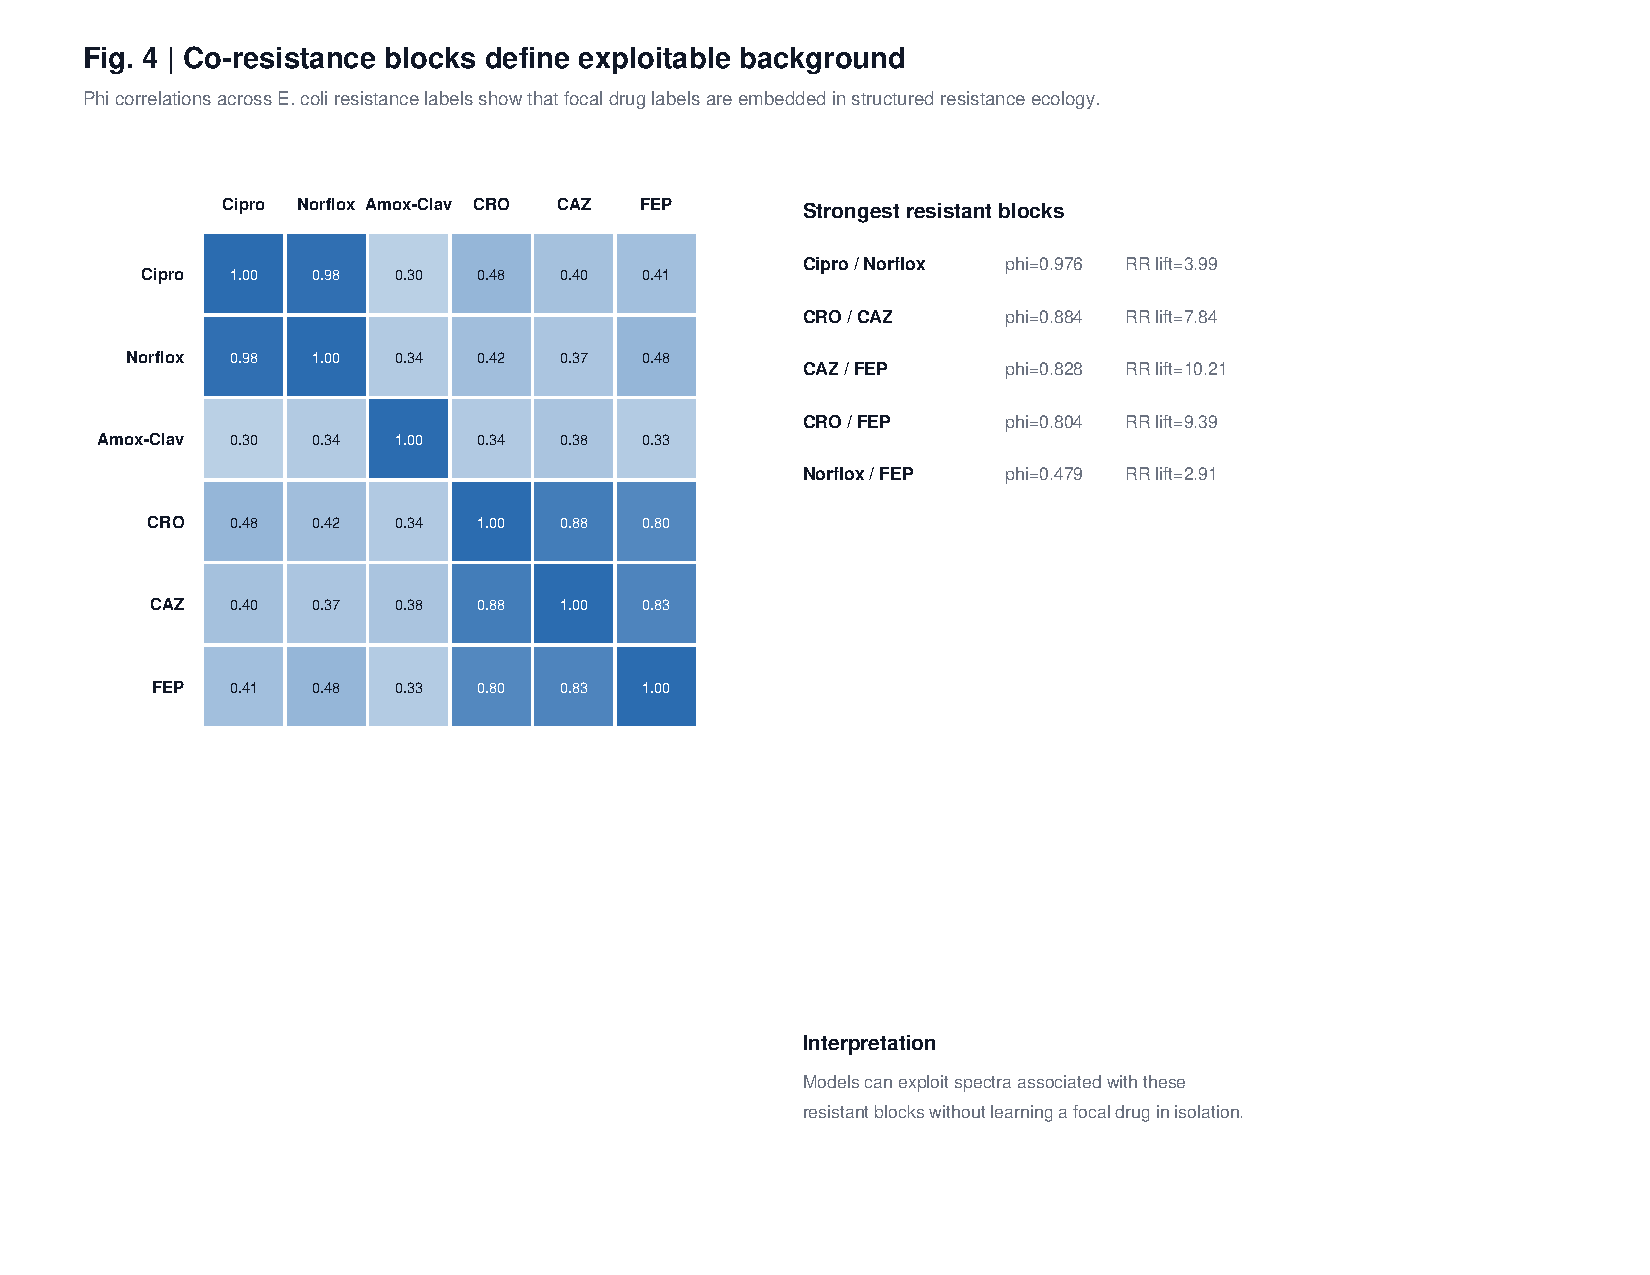
\includegraphics[width=\linewidth]{figure_4_cross_resistance_network.pdf}
\caption{Cross-resistance structure}
\end{subfigure}
\hfill
\begin{subfigure}{0.48\linewidth}
\centering
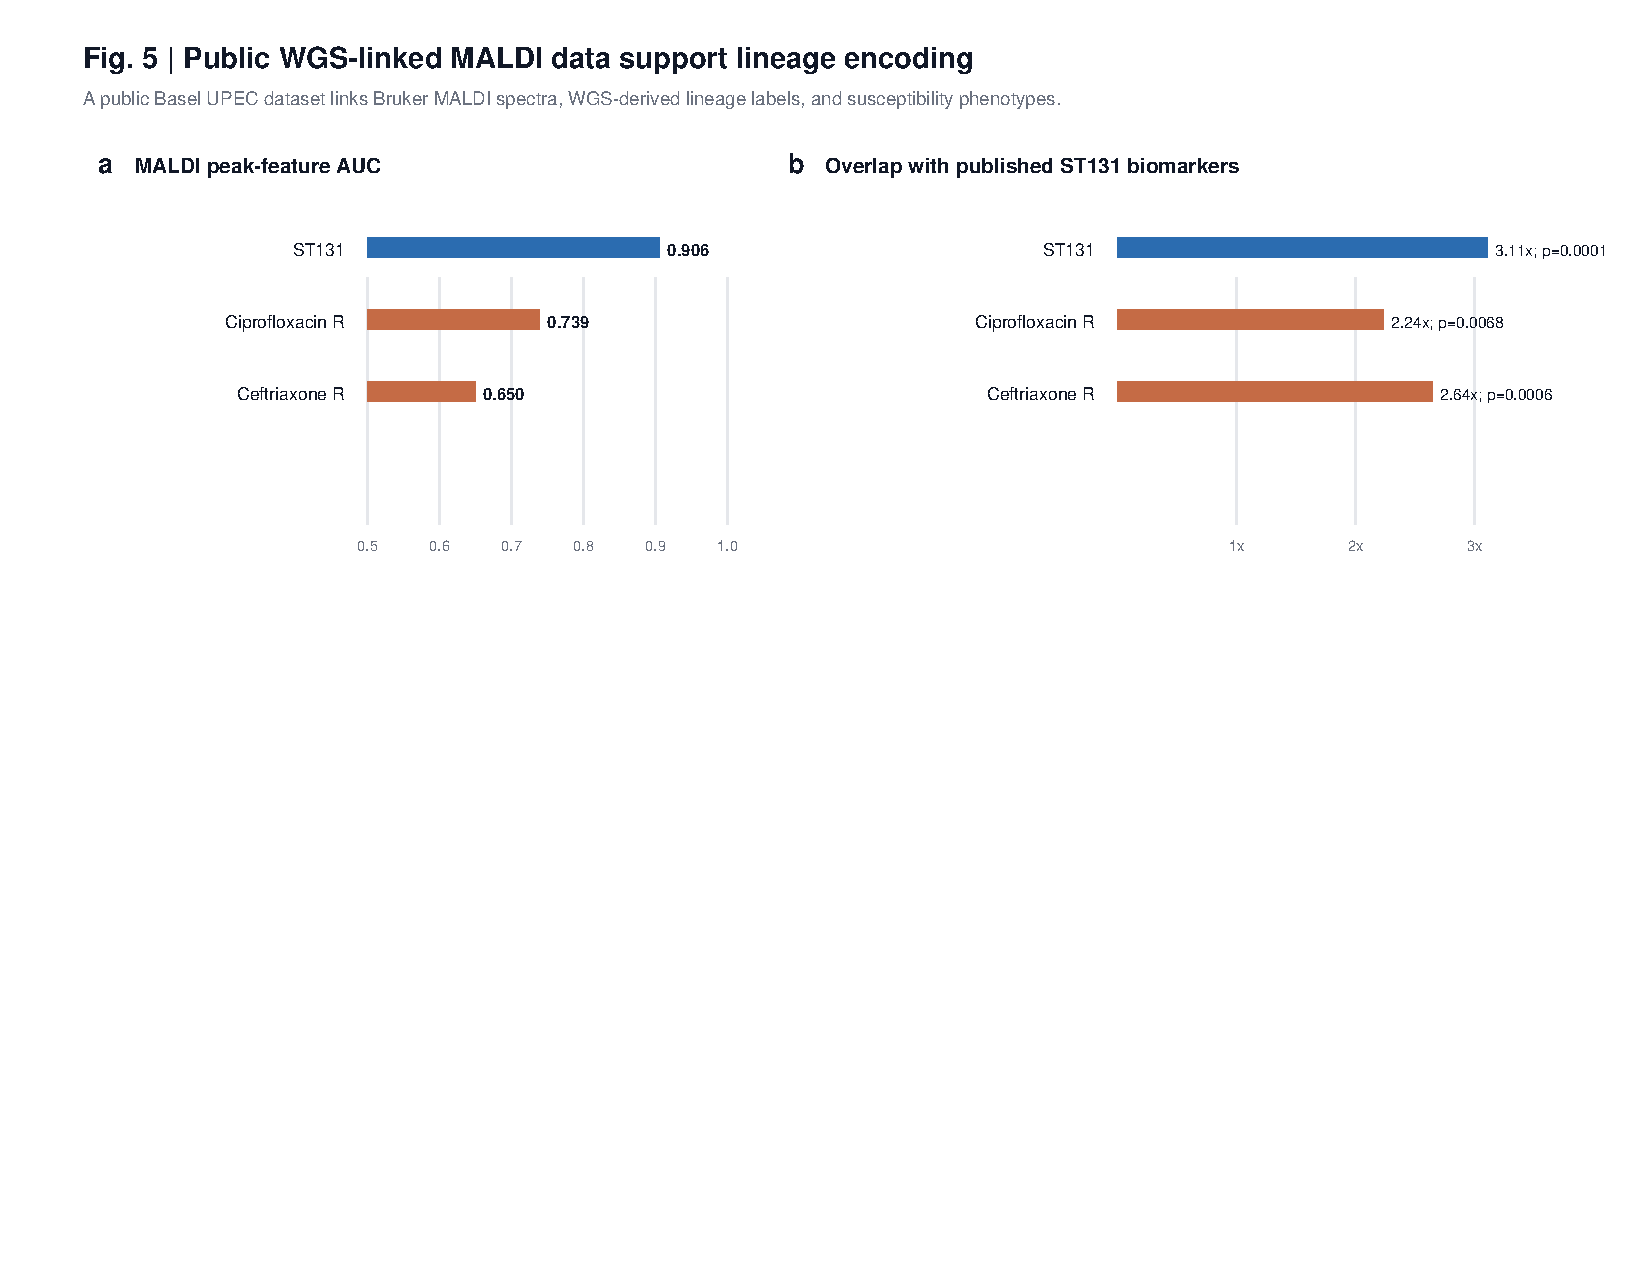
\includegraphics[width=\linewidth]{figure_5_public_wgs_proteomic_support.pdf}
\caption{WGS-linked MALDI support}
\end{subfigure}
\caption{\textbf{Resistant-population background is phenotypically and spectrally structured.} Cross-resistance networks show strong exploitable label blocks in the \textit{E.~coli} AST panel. Public WGS-linked MALDI data show that ST131 lineage is highly predictable from MALDI peak features and that resistance-associated discriminative bins are enriched for published ST131 biomarker mass neighborhoods.}
\label{fig:background-support}
\end{figure}

\subsection*{Stress tests defined the boundary of the claim}

We ran two additional analyses to define what the framework can and cannot claim. First, falsification controls compared observed model AUC with a background-burden-only score and a within-background shuffled-label null. In the audited stress-test rows, no row exceeded both controls, and only a small subset exceeded the shuffle null while remaining competitive with the burden-only control. These controls make the interpretation conservative: high raw AUC should not be treated as focal-drug evidence unless it survives background-aware comparisons.

Second, we used MARISMa as an external stress test. MARISMa is an independent MALDI-TOF/AST resource with replicate spot-level spectra and a different collection context from DRIAMS. We aggregated MARISMa spot-level predictions to isolate-drug rows and audited the resulting external predictions for the same \textit{E.~coli} six-drug panel. The locked DRIAMS-trained model showed weak raw signal across all six targets, with raw AUCs near chance. This is a transfer failure, not a successful external validation. It is useful because it shows how the audit should be used in practice: when raw performance is weak, the correct conclusion is failed transfer before any more nuanced background interpretation.

\section*{Discussion}

This study shows that MALDI-TOF AMR prediction should not be interpreted from raw external AUC alone. In the DRIAMS \textit{E.~coli} panel, ciprofloxacin predictions retained measurable but site-dependent within-background signal after matching by co-resistance context, whereas amoxicillin-clavulanic acid weakened or collapsed at external sites. In a second organism-drug setting, \textit{S.~aureus}/oxacillin retained background-matched signal at the evaluable DRIAMS sites. Exact co-resistance-only baselines showed that several focal resistance labels were predictable from non-focal AST labels alone, making explicit the shortcut structure that raw MALDI AUC can obscure. Together, these results support a practical conclusion: MALDI-TOF AMR models are background-sensitive predictors, and their evaluation should report how much performance survives resistant-population background control.

The main contribution is not the observation that bacterial population structure exists. That is well established in microbial genomics and AMR prediction\cite{yu2025population}. The contribution is an operational audit that can be applied to any fixed MALDI-TOF AMR prediction table. The audit converts a vague concern, ``maybe the model learned the resistant clone,'' into row-level quantities: raw AUC, matched AUC, background-centered AUC, pairwise within-background accuracy, matched retention, and adequacy labels. It complements spectral hierarchical stratification by moving the test from the raw-spectrum/split-design level to the prediction-table/reporting level\cite{weis2022stratification}. In that sense, the audit is best viewed as a MALDI-AMR-specific extension to transparent clinical prediction-model reporting: TRIPOD+AI and PROBAST define what should be reported and appraised for clinical prediction models, while background matching adds a domain-specific check for resistant-population background sensitivity\cite{collins2024tripodai,wolff2019probast}.

The co-resistance-only baseline clarifies what the background-matched audit controls. A model can appear useful when the focal drug label is predictable from the rest of the AST panel, even before spectra are considered. This was especially visible in \textit{E.~coli}: DRIAMS-C ciprofloxacin and amoxicillin-clavulanic acid had exact-background-only AUCs of 0.918 and 0.687, respectively, while the MALDI centered AUCs were 0.646 and 0.497. The \textit{S.~aureus}/oxacillin result did not simply reproduce that pattern. At A-2018 and DRIAMS-C, MALDI predictions retained centered signal that was competitive with or higher than the exact-background-only baseline. This does not prove mecA detection or mechanism; it shows that the audit can separate AST-ecology-dominated rows from rows where MALDI scores retain signal after matching.

The ciprofloxacin result should be interpreted carefully. Retained within-background signal does not prove that the model learned a biochemical fluoroquinolone resistance mechanism. Ciprofloxacin resistance is linked to ST131 and other fluoroquinolone-resistant \textit{E.~coli} lineages, and MALDI can encode lineage-associated protein variation. The audit only shows that after matching on the observed co-resistance panel, some ranking signal remains. The norfloxacin composition check sharpens this interpretation. At the interpretable sites, the retained ciprofloxacin signal was not obtained by comparing resistant and susceptible isolates inside an almost redundant norfloxacin-susceptible background. It was obtained after matching on available beta-lactam and cephalosporin backgrounds, meaning the model retained partial ciprofloxacin ranking across a different drug-class ecology. That is stronger evidence of drug-specific residual signal than the anticipated fluoroquinolone-pair control would have provided, although the remaining signal may still reflect focal biology, residual lineage not captured by the AST signature, or both. The DRIAMS-D result is especially informative: high matched retention but only weak centered AUC suggests that ciprofloxacin-associated spectral structure did not transfer uniformly to that site. Because DRIAMS-D was contributed by a laboratory service provider rather than the same hospital ecology as the training site\cite{weis2022driams}, this attenuation is consistent with the audit detecting a shift in resistant-population background rather than a uniform ciprofloxacin signature. This is why the paper reports pairwise within-background accuracy, matched retention, and threshold sensitivity instead of presenting centered AUC as proof of mechanism.

The amoxicillin-clavulanic acid result is more directly actionable. At external sites with high matched retention, performance approached chance after background adjustment. A model with that behavior should not be interpreted as a robust focal-drug predictor simply because raw AUC is above chance in some sites. The \textit{S.~aureus}/oxacillin result is the complementary case: the audit found retained signal rather than collapse, which is consistent with oxacillin resistance being concentrated in structured MRSA/MSSA backgrounds while still leaving measurable within-background discrimination. For clinical microbiology, this is the point of the audit: it identifies when apparent transfer is likely to depend on the distribution of resistant populations in the test site and when a model retains signal after that observable distribution is controlled.

The public WGS-linked UPEC analysis provides biological grounding but not direct DRIAMS lineage proof. It shows that MALDI peak features can identify ST131 very strongly and that resistance predictions are attenuated when sequence-type background is controlled. Because those isolates are independent of the DRIAMS benchmark, this analysis should be read as mechanistic plausibility and external support, not as evidence that the DRIAMS model detected ST131 in the primary data.

Several limitations are important. First, co-resistance background is only a proxy for population background. Isolates with identical AST signatures can differ by sequence type, plasmid content, and resistance mechanism. DRIAMS-linked WGS or MLST would allow direct lineage-centered decomposition. Second, background-centered AUC is a pooled residual statistic, not a purely within-stratum statistic; that is why pairwise within-background accuracy is reported as the strict companion metric. Third, sparse matched strata limit interpretation for some drug-site rows, especially cephalosporins and smaller site panels. This is why the DRIAMS-B \textit{S.~aureus}/oxacillin row is described as supportive but sparse: it had one valid stratum at the main threshold and no valid strata at the stricter threshold of ten per class. Fourth, norfloxacin missingness prevents a fully controlled fluoroquinolone-pair analysis at A-2018, DRIAMS-C, and DRIAMS-D, even though it also means the interpretable ciprofloxacin audit is a cross-class beta-lactam/cephalosporin background test. Fifth, mass-bin enrichment against published ST131 biomarker masses does not identify proteins. Sixth, the Weis/Borgwardt analysis supports official LR parity only for the limited upstream panel already checked, while the broader six-drug export is a background-audit stress test rather than an exact replication claim. Seventh, the multi-organism extension remains limited to one additional organism-drug case. \textit{S.~aureus}/oxacillin strengthens the framework beyond an \textit{E.~coli}-only case study, but an atlas-scale analysis across many organism-drug pairs is still needed before claiming comprehensive MALDI-AMR behavior across DRIAMS.

For the field, the implication is straightforward. MALDI-TOF AMR studies should report background-centered AUC, pairwise within-background accuracy, matched retention, and a cross-resistance summary alongside raw AUC. A model should be considered deployment-ready for a drug-site context only when its predictions survive the observable resistant-population background available in that context. This standard would not eliminate the need for prospective clinical validation, but it would make preclinical and retrospective validation more honest about what the model may have learned.

\section*{Methods}

\subsection*{Primary DRIAMS data and evaluation design}

We used the DRIAMS MALDI-TOF and AST resource as the primary clinical benchmark\cite{weis2022driams,driamsdryad}. Models were trained on DRIAMS-A isolates collected before 2018 and evaluated on a temporal DRIAMS-A 2018 holdout and the external DRIAMS-B, DRIAMS-C, and DRIAMS-D sites. The primary organism panel was \textit{E.~coli}. The six-drug \textit{E.~coli} panel included ciprofloxacin, norfloxacin, amoxicillin-clavulanic acid, ceftriaxone, ceftazidime, and cefepime. The second organism-drug analysis used a seven-drug \textit{S.~aureus} panel with oxacillin as the primary target and penicillin, ciprofloxacin, erythromycin, clindamycin, gentamicin, and fusidic acid as non-focal background labels. Intermediate AST labels and isolates missing the focal-drug label were excluded from the corresponding focal-drug evaluation. The \textit{S.~aureus} DRIAMS-D export contained no usable oxacillin focal rows, so DRIAMS-D was not included in the \textit{S.~aureus}/oxacillin site-level claim.

\subsection*{Prediction models}

The primary model was a multi-task convolutional neural network trained on MALDI-TOF spectra represented over the 2,000 to 20,000 m/z range. The \textit{S.~aureus}/oxacillin predictions were generated from the same multi-task CNN workflow applied to the \textit{S.~aureus} drug panel. A multi-task LightGBM model trained on peak-bin features from the same general spectral range was used as an architecture check. The LightGBM analysis was not intended to optimize performance; it tested whether background sensitivity appeared outside the neural-network model. Weis/Borgwardt-style logistic regression outputs were exported separately with an ID-preserving pipeline and audited as supplementary published-workflow compatibility evidence.

\subsection*{Background signatures}

For each isolate and focal drug, the co-resistance background signature was the concatenation of the binary AST labels for all non-focal drugs in the same organism panel. For ciprofloxacin, for example, the signature encoded norfloxacin, amoxicillin-clavulanic acid, ceftriaxone, ceftazidime, and cefepime labels. The focal drug was never included in its own background signature. A valid stratum required at least three resistant and three susceptible isolates for the focal drug. Strata failing this threshold were excluded from matched and centered performance estimates and counted against matched retention.

\subsection*{Audit metrics}

Raw AUC was computed from all available focal-drug prediction rows in a site. Matched AUC was computed after restricting to valid background strata. Background-centered AUC was computed by subtracting the mean model score within each valid stratum from each isolate score, then recomputing AUC from the pooled residual scores. Pairwise within-background accuracy was computed from resistant-susceptible pairs within the same valid stratum and measured the fraction of pairs in which the resistant isolate received the higher model score; ties counted as 0.5. Matched retention was the fraction of focal-drug rows retained in valid strata.

\subsection*{Co-resistance-only baseline}

For each focal drug-site row, we computed a non-spectral baseline that predicted focal resistance from the complete non-focal AST background signature only. For each isolate, the exact-background score was the leave-one-out smoothed prevalence of focal resistance among other isolates with the same non-focal AST signature:
\[
  \hat{p}_{i} = \frac{r_{-i} + \alpha p_{\mathrm{global}}}{n_{-i} + \alpha},
\]
where $r_{-i}$ and $n_{-i}$ are the resistant count and total count in the isolate's background stratum after excluding the isolate itself, $p_{\mathrm{global}}$ is the site-drug focal resistance prevalence, and $\alpha=2$ is the smoothing parameter. We also computed a simpler burden-only score equal to the number of resistant non-focal drug labels. These baselines used no MALDI spectra and no model probability. They are diagnostic controls for shortcut structure, not pretreatment clinical models, because they require the non-focal AST panel.

\subsection*{Uncertainty and adequacy labels}

Bootstrap confidence intervals were computed with 500 resamples. Permutation p-values for the raw-to-centered drop were computed by shuffling focal-drug labels within valid background strata and recomputing centered AUC over 500 permutations. Rows with no valid strata were labeled not interpretable. Rows with very small matched sample counts or low matched retention were labeled cautionary and were not used as primary evidence even when centered AUC was high.

\subsection*{Revision sensitivity analyses}

To address the ciprofloxacin/norfloxacin circularity concern, we parsed each valid ciprofloxacin background signature and summarized whether the norfloxacin component was resistant, susceptible, unknown, or absent. This check was repeated at valid-stratum thresholds of at least three, five, and ten resistant and susceptible isolates. To test whether the primary ciprofloxacin versus amoxicillin-clavulanic acid contrast depended on the permissive threshold of three per class, we reran the audit at thresholds of five and ten per class with the same prediction rows and background signatures. These sensitivity analyses were descriptive and did not rerun model training.

\subsection*{Cross-resistance network}

For each pair of drugs in the \textit{E.~coli} panel, we computed phi correlation, resistant-resistant lift, and resistant Jaccard similarity from isolate-level binary AST labels among isolates with both labels known. These measures described the label ecology available to AMR prediction models and identified co-resistance blocks that could serve as background signal.

\subsection*{Public WGS-linked UPEC support analysis}

We analyzed public Basel uropathogenic \textit{E.~coli} resources linking WGS metadata and Bruker MALDI-derived peak features\cite{cuenod2023papgii}. The analysis included 407 isolates with complete usable peak features and metadata after manifest joining; 55 were ST131 by WGS-derived sequence type. We created 50 Da-binned MALDI peak features and evaluated centroid-direction classifiers for ST131 identity, ciprofloxacin resistance, and ceftriaxone resistance using five cross-validation folds. To estimate lineage-controlled resistance signal, we computed centered AUCs after subtracting WGS-derived background group means, including exact sequence type. Sequence-type-centered analyses retained only groups containing both resistant and susceptible isolates for the focal phenotype.

\subsection*{Published ST131 biomarker enrichment}

Published ST131 MALDI biomarker masses were taken from Nakamura \textit{et al.}\cite{nakamura2019st131}. For each target, we ranked MALDI bins by absolute mean log-intensity difference between positive and negative isolates and selected the top 75 bins. We counted overlaps within 40 Da of published ST131 biomarker masses and compared observed overlap with a mass-stratified permutation null. Individual mass-bin matches were interpreted as spectral-neighborhood overlaps only. They were not treated as protein identifications.

\subsection*{Falsification controls}

For each audited drug-site row, we compared observed model AUC with a background-burden-only score, defined as the number of resistant non-focal drug labels in the isolate's panel. We also generated a within-background shuffled-label null by permuting focal-drug labels within valid background strata. These controls were used to assess whether observed raw performance exceeded simple background-derived alternatives.

\subsection*{MARISMa stress test}

MARISMa predictions were generated at spot level and aggregated before auditing to avoid treating replicate spectra as independent isolates. Rows were grouped by site, year, isolate identifier, organism, and drug. The isolate-drug probability was the mean of replicate spot probabilities. Groups with conflicting binary labels were excluded and written to a duplicate-handling report. The committed stress-test snapshot collapsed 9,597 spot-level rows to 6,022 isolate-drug rows and excluded 20 conflicting isolate-drug groups before auditing.

\subsection*{Software and reproducibility}

All analyses operate on a flat prediction table with isolate identifier, site, year, organism, drug, binary AST label, and model probability. The main audit engine is \texttt{run\_background\_audit\_framework.py}. Publication outputs are generated by \texttt{scripts/make\_final\_framework\_tables\_figures.py} and related figure scripts. Weis/Borgwardt published-code prediction exports are produced by \texttt{scripts/export\_weis\_predictions\_for\_audit.py} and parity checks by \texttt{scripts/compare\_weis\_raw\_metrics.py}. The critique-driven ciprofloxacin/norfloxacin composition and threshold sensitivity checks are generated by \texttt{scripts/revision\_audit\_checks.py}. The AST-only control baselines are generated by \texttt{scripts/co\_resistance\_only\_baseline.py}. Derived outputs are written under \texttt{outputs/analysis\_outputs/}.

\section*{Data availability}

Raw DRIAMS spectra and AST labels are available from the DRIAMS Dryad release\cite{driamsdryad}. Public WGS-linked UPEC resources are available through the Cuenod \textit{et al.} study resources\cite{cuenod2023papgii}. Derived summary tables and figure source data are included in this repository under \texttt{outputs/final\_framework\_outputs/}, \texttt{outputs/analysis\_outputs/}, and \texttt{manuscript/source\_data/}.

\section*{Code availability}

Analysis code is available at \url{https://github.com/byungkim113/background-matched-maldi-amr-audit}, including the model-agnostic audit engine, prediction exporters, public WGS-linked MALDI support analyses, source-data tables, and figure-generation scripts.

\section*{Acknowledgements}

We thank the DRIAMS investigators and the public UPEC WGS/MALDI data generators for releasing resources that make independent evaluation possible.

\section*{Author contributions}

B.K. conceived the audit framework, implemented the analyses, generated outputs, and drafted the manuscript. Additional author contributions should be completed and approved before submission.

\section*{Competing interests}

The authors declare no competing interests. This statement should be confirmed by all authors before submission.

\begin{thebibliography}{99}

\bibitem{murray2022amr}
Murray, C. J. L. \textit{et al.} Global burden of bacterial antimicrobial resistance in 2019: a systematic analysis. \textit{Lancet} \textbf{399}, 629--655 (2022).

\bibitem{seng2009maldi}
Seng, P. \textit{et al.} Ongoing revolution in bacteriology: routine identification of bacteria by matrix-assisted laser desorption ionization time-of-flight mass spectrometry. \textit{Clin. Infect. Dis.} \textbf{49}, 543--551 (2009).

\bibitem{patel2015maldi}
Patel, R. MALDI-TOF MS for the diagnosis of infectious diseases. \textit{Clin. Chem.} \textbf{61}, 100--111 (2015).

\bibitem{weis2022driams}
Weis, C. \textit{et al.} Direct antimicrobial resistance prediction from clinical MALDI-TOF mass spectra using machine learning. \textit{Nat. Med.} \textbf{28}, 164--174 (2022).

\bibitem{driamsdryad}
Weis, C. \textit{et al.} DRIAMS: Database of Resistance Information on Antimicrobials and Mass Spectra. Dryad. \url{https://doi.org/10.5061/dryad.bzkh1899q} (2022).

\bibitem{msdeepamr2024}
Lopez-Cortes, X. A., Manriquez-Troncoso, J. M., Hernandez-Garcia, R. \& Peralta, D. MSDeepAMR: antimicrobial resistance prediction based on deep neural networks and transfer learning. \textit{Front. Microbiol.} \textbf{15}, 1361795 (2024).

\bibitem{multilabel2024}
Astudillo, C. A., Lopez-Cortes, X. A., Ocque, E. \textit{et al.} Multi-label classification to predict antibiotic resistance from raw clinical MALDI-TOF mass spectrometry data. \textit{Sci. Rep.} \textbf{14}, 31283 (2024).

\bibitem{saureus2024}
Wang, W.-Y., Chiu, C.-F., Tsao, S.-M., Lee, Y.-L. \& Chen, Y.-H. Accurate prediction of antimicrobial resistance and genetic marker of \textit{Staphylococcus aureus} clinical isolates using MALDI-TOF MS and machine learning -- across DRIAMS and Taiwan database. \textit{Int. J. Antimicrob. Agents} \textbf{64}, 107329 (2024).

\bibitem{canton2011coresistance}
Canton, R. \& Ruiz-Garbajosa, P. Co-resistance: an opportunity for the bacteria and resistance genes. \textit{Curr. Opin. Pharmacol.} \textbf{11}, 477--485 (2011).

\bibitem{pal2015coselection}
Pal, C., Bengtsson-Palme, J., Kristiansson, E. \& Larsson, D. G. J. Co-occurrence of resistance genes to antibiotics, biocides and metals reveals novel insights into their co-selection potential. \textit{BMC Genomics} \textbf{16}, 964 (2015).

\bibitem{yu2025population}
Yu, Y., Wheeler, N.~E. \& Barquist, L. Biased sampling driven by bacterial population structure confounds machine learning prediction of antimicrobial resistance. \textit{PLOS Biol.} \textbf{23}, e3003539 (2025).

\bibitem{collins2024tripodai}
Collins, G. S., Moons, K. G. M., Dhiman, P., Riley, R. D., Beam, A. L., Van Calster, B. \textit{et al.} TRIPOD+AI statement: updated guidance for reporting clinical prediction models that use regression or machine learning methods. \textit{BMJ} \textbf{385}, e078378 (2024).

\bibitem{wolff2019probast}
Wolff, R. F., Moons, K. G. M., Riley, R. D., Whiting, P. F., Westwood, M., Collins, G. S. \textit{et al.} PROBAST: a tool to assess the risk of bias and applicability of prediction model studies. \textit{Ann. Intern. Med.} \textbf{170}, 51--58 (2019).

\bibitem{weis2022stratification}
Weis, C., Rieck, B.~A., Balzer, S., Cuenod, A., Egli, A. \& Borgwardt, K. Improved MALDI-TOF MS based antimicrobial resistance prediction through hierarchical stratification. \textit{bioRxiv} \url{https://doi.org/10.1101/2022.04.13.488198} (2022).

\bibitem{rosenbaum1983propensity}
Rosenbaum, P. R. \& Rubin, D. B. The central role of the propensity score in observational studies for causal effects. \textit{Biometrika} \textbf{70}, 41--55 (1983).

\bibitem{cuenod2023papgii}
Cuenod, A. \textit{et al.} Bacterial genome-wide association study substantiates \textit{papG}II of \textit{Escherichia coli} as a major risk factor for urosepsis. \textit{Genome Med.} \textbf{15}, 89 (2023).

\bibitem{nicolas2014st131}
Nicolas-Chanoine, M.-H., Bertrand, X. \& Madec, J.-Y. \textit{Escherichia coli} ST131, an intriguing clonal group. \textit{Clin. Microbiol. Rev.} \textbf{27}, 543--574 (2014).

\bibitem{nakamura2019st131}
Nakamura, A. \textit{et al.} Identification of specific protein amino acid substitutions of extended-spectrum beta-lactamase-producing \textit{Escherichia coli} ST131: a proteomics approach using mass spectrometry. \textit{Sci. Rep.} \textbf{9}, 8555 (2019).

\bibitem{domainadapt2026}
Chen, M.-I., Hsu, Y.-L. \& Chen, Y.-H. Benchmarking domain adaptation methods for cross-site antimicrobial resistance prediction from MALDI-TOF mass spectrometry data. \textit{Comput. Biol. Chem.} \textbf{124}, 109097 (2026).

\bibitem{planet2017st8}
Strau{\ss}, L. \textit{et al.} Origin, evolution, and global transmission of community-acquired \textit{Staphylococcus aureus} ST8. \textit{Proc. Natl. Acad. Sci. U.S.A.} \textbf{114}, E10596--E10604 (2017).

\bibitem{diep2006usa300}
Diep, B. A. \textit{et al.} Complete genome sequence of USA300, an epidemic clone of community-acquired meticillin-resistant \textit{Staphylococcus aureus}. \textit{Lancet} \textbf{367}, 731--739 (2006).

\end{thebibliography}

\end{document}
